% This is "sig-alternate.tex" V2.1 April 2013
% This file should be compiled with V2.5 of "sig-alternate.cls" May 2012
%
% This example file demonstrates the use of the 'sig-alternate.cls'
% V2.5 LaTeX2e document class file. It is for those submitting
% articles to ACM Conference Proceedings WHO DO NOT WISH TO
% STRICTLY ADHERE TO THE SIGS (PUBS-BOARD-ENDORSED) STYLE.
% The 'sig-alternate.cls' file will produce a similar-looking,
% albeit, 'tighter' paper resulting in, invariably, fewer pages.
%
% ----------------------------------------------------------------------------------------------------------------
% This .tex file (and associated .cls V2.5) produces:
%       1) The Permission Statement
%       2) The Conference (location) Info information
%       3) The Copyright Line with ACM data
%       4) NO page numbers
%
% as against the acm_proc_article-sp.cls file which
% DOES NOT produce 1) thru' 3) above.
%
% Using 'sig-alternate.cls' you have control, however, from within
% the source .tex file, over both the CopyrightYear
% (defaulted to 200X) and the ACM Copyright Data
% (defaulted to X-XXXXX-XX-X/XX/XX).
% e.g.
% \CopyrightYear{2007} will cause 2007 to appear in the copyright line.
% \crdata{0-12345-67-8/90/12} will cause 0-12345-67-8/90/12 to appear in the copyright line.
%
% ---------------------------------------------------------------------------------------------------------------
% This .tex source is an example which *does* use
% the .bib file (from which the .bbl file % is produced).
% REMEMBER HOWEVER: After having produced the .bbl file,
% and prior to final submission, you *NEED* to 'insert'
% your .bbl file into your source .tex file so as to provide
% ONE 'self-contained' source file.
%
% ================= IF YOU HAVE QUESTIONS =======================
% Questions regarding the SIGS styles, SIGS policies and
% procedures, Conferences etc. should be sent to
% Adrienne Griscti (griscti@acm.org)
%
% Technical questions _only_ to
% Gerald Murray (murray@hq.acm.org)
% ===============================================================
%
% For tracking purposes - this is V2.0 - May 2012

\documentclass{sig-alternate-05-2015}


\begin{document}

% Copyrightsetcopyright{acmcopyright}
%\setcopyright{acmlicensed}
%\setcopyright{rightsretained}
%\setcopyright{usgov}
%\setcopyright{usgovmixed}
%\setcopyright{cagov}
%\setcopyright{cagovmixed}


%
% --- Author Metadata here ---
\conferenceinfo{SCC}{2017 Denver, CO USA}
%\CopyrightYear{2007} % Allows default copyright year (20XX) to be over-ridden - IF NEED BE.
%\crdata{0-12345-67-8/90/01}  % Allows default copyright data (0-89791-88-6/97/05) to be over-ridden - IF NEED BE.
% --- End of Author Metadata ---

\title{Reproducing The Vectorization of the Tersoff Multi-Body Potential:  An Exercise in Performance Portability for SC17}
%
% You need the command \numberofauthors to handle the 'placement
% and alignment' of the authors beneath the title.
%
% For aesthetic reasons, we recommend 'three authors at a time'
% i.e. three 'name/affiliation blocks' be placed beneath the title.
%
% NOTE: You are NOT restricted in how many 'rows' of
% "name/affiliations" may appear. We just ask that you restrict
% the number of 'columns' to three.
%
% Because of the available 'opening page real-estate'
% we ask you to refrain from putting more than six authors
% (two rows with three columns) beneath the article title.
% More than six makes the first-page appear very cluttered indeed.
%
% Use the \alignauthor commands to handle the names
% and affiliations for an 'aesthetic maximum' of six authors.
% Add names, affiliations, addresses for
% the seventh etc. author(s) as the argument for the
% \additionalauthors command.
% These 'additional authors' will be output/set for you
% without further effort on your part as the last section in
% the body of your article BEFORE References or any Appendices.

\numberofauthors{6} %  in this sample file, there are a *total*
% of EIGHT authors. SIX appear on the 'first-page' (for formatting
% reasons) and the remaining two appear in the \additionalauthors section.
%
\author{
% You can go ahead and credit any number of authors here,
% e.g. one 'row of three' or two rows (consisting of one row of three
% and a second row of one, two or three).
%
% The command \alignauthor (no curly braces needed) should
% precede each author name, affiliation/snail-mail address and
% e-mail address. Additionally, tag each line of
% affiliation/address with \affaddr, and tag the
% e-mail address with \email.
%
% 1st. author
\alignauthor
Janaan Lake\\
       \affaddr{University of Utah}\\
       \email{janaanl@hotmail.com}
% 2nd. author
\alignauthor
Qixiang Chao\\
       \affaddr{University of Utah}\\
       \email{cqx820@foxmail.com}
% 3rd. author
\alignauthor Hannah Eyre\\
       \affaddr{University of Utah}\\
       \email{hannahreyre@gmail.com}
\and  % use '\and' if you need 'another row' of author names
% 4th. author
\alignauthor Emerson Ford\\
		\affaddr{University of Utah}\\
       \email{emersontford@gmail.com}
% 5th. author
\alignauthor Kevin Parker\\
		\affaddr{University of Utah}\\
       \email{kevin.m.parker@gmail.com}
% 6th. author
\alignauthor Kincaid Savoie\\
		\affaddr{University of Utah}\\
       \email{kincaidsavioe@gmail.com}
}
% There's nothing stopping you putting the seventh, eighth, etc.
% author on the opening page (as the 'third row') but we ask,
% for aesthetic reasons that you place these 'additional authors'
% in the \additional authors block, viz.

% Just remember to make sure that the TOTAL number of authors
% is the number that will appear on the first page PLUS the
% number that will appear in the \additionalauthors section.

\maketitle
\begin{abstract}
This paper describes our SC17 Student Cluster Competition team's efforts to reproduce the results of an SC16 paper titled The Vectorization of the Tersoff Multi-Body Potential:  An Exercise in Performance Portability. This application optimizes the Tersoff potential within the molecular dynamics code LAMMPS and provides portability for these optimizations across architectures.  Our results demonstrated that we could reproduce almost all of the results in the original publication. We expect the different datasets and differences in our cluster configuration to account for the variation in some of the results.
\end{abstract}
%
\section{Introduction}
The ability to reproduce results is essential to advancing algorithms and optimizations suitable for high-performance computing.  At the SC17 conference, a component of the Student Cluster Competition required teams to reproduce the results from a prior conference by reading a paper and installing the associated software on their cluster.  The overall competition involves a team of six undergraduates designing a new cluster from state-of-the-art hardware and software, running a set of required applications on the hardware, and providing written and oral descriptions of the results. This paper presents the results of the reproducibility exercise from SC16, using results that were collected during the conference.  

Molecular dynamics simulations consume a significant portion of the supercomputing cycles around the world.  The selected paper describes an approach to extending the LAMMPS molecular dynamic simulator with a new, optimized and portable implementation of the Tersoff multi-body potential.  These  include scalar optimizations and vectorization.  The vectorization optimizations include mapping the outer loops to different execution schemes, avoiding masking, and filtering neighbor lists.   

We are testing the portability and speedups of these optimizations on our cluster using tests run on a single processor, one node and across all four nodes of our cluster.  
\section{Cluster and Software Details}
Our team partnered with Dell, Nvidia and Intel to build the cluster.  The resulting system has one Dell PowerEdge R730 head node and four Dell PowerEdge R740s compute nodes. The head node has two Intel Xeon E5-2680 v4 CPUs clocked at 2.4 GHz and supports AVX2 instruction sets.  Each compute node has two Intel Xeon Gold 6130 CPUs clocked at 2.10 GHz and supports AVX-512 instruction sets. The head node has 2 sockets with 14 cores and 128GB memory for each socket. The computes nodes have 2 sockets with 16 cores, and each socket has 96 GB of memory.  For the interconnect, we use Mellanox EDR. The cluster runs CentOS 7 with Linux kernel version 3.10.0-693.2.2.el7.x86\_64.

To compile LAMMPS, we cloned the repository from GitHub at \texttt{https://github.com/HPAC/lammps-tersoff-vector}.  We used the LAMMPS version 10Mar16 that was provided in this repository.  We modified the build script in the aices-westmere folder for our architecture and used code from the USER-INTEL package.  Prior to the competition we used Intel 18.0 and Intel MPI 5.1.3 to build the binaries.

\section{Results}
Because our cluster is heterogeneous, we tested the optimizations on both vector instruction sets supported on our cluster:  AVX2, and AVX-512. We were provided four data sets to use for the test runs:  \texttt{in.tersoff, in.tersoff\_bench, in.tersoff-acc} and \texttt{in.porter}. 

\subsection{Accuracy Test}
The LAMMPS code uses double precision floating point operations.  The optimized code provided implementations to compute the Tersoff potential using single and mixed precision. To validate the reduced precision implementations, the difference in energy was measured during long-running simulations.  We compared the results of two long-running simulations tests, comparing the accuracy of the double precision with the mixed precision and the accuracy of the double precision with the single precision.  We used the \texttt{in.tersoff-acc} data set.  These tests were run on one of our compute nodes using the AVX-512 instruction set, and the results can be seen in Figures 1 and 2.   

Our results diverged from those in the paper as the relative difference increased over the number of timesteps.  

\begin{figure}
\centering
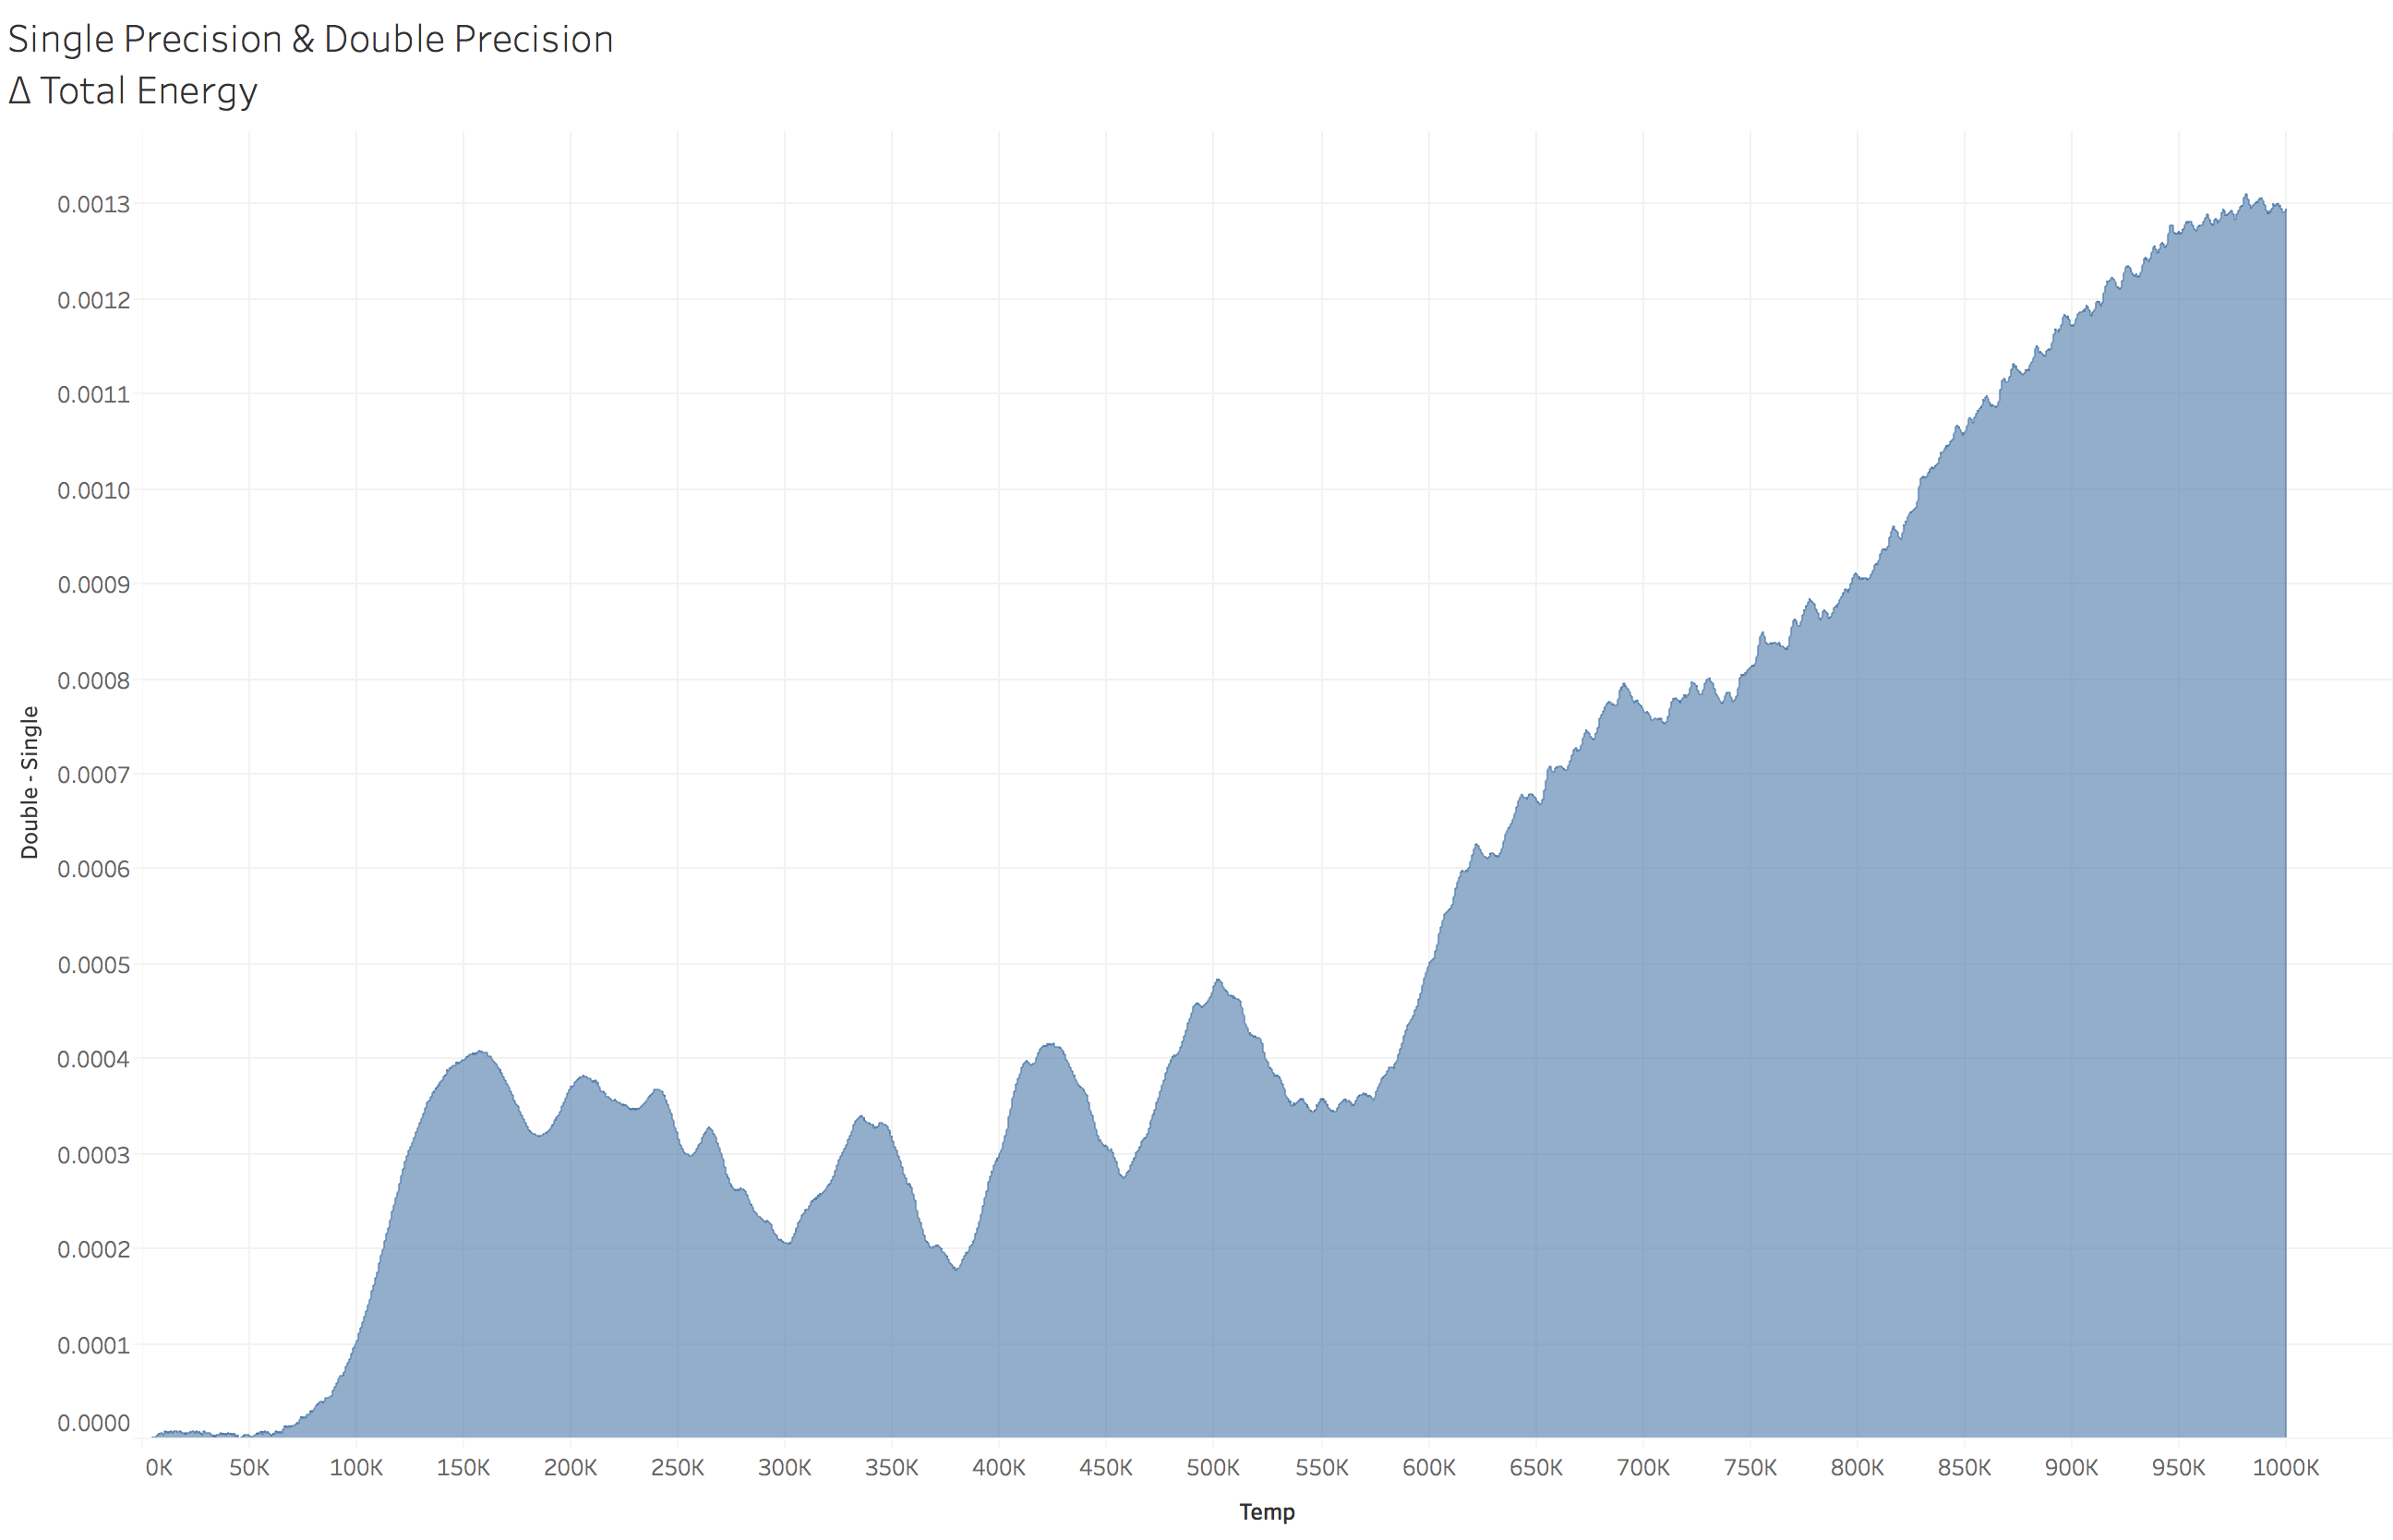
\includegraphics[height=6cm, width=8cm]{Single-Double.png}
\caption{Validation of the single precision solver: relative difference between the single and double precision solvers for a system of 32,000 atoms for $10^{6}$ timesteps}
\vskip -6pt
\end{figure}

\begin{figure}
\centering
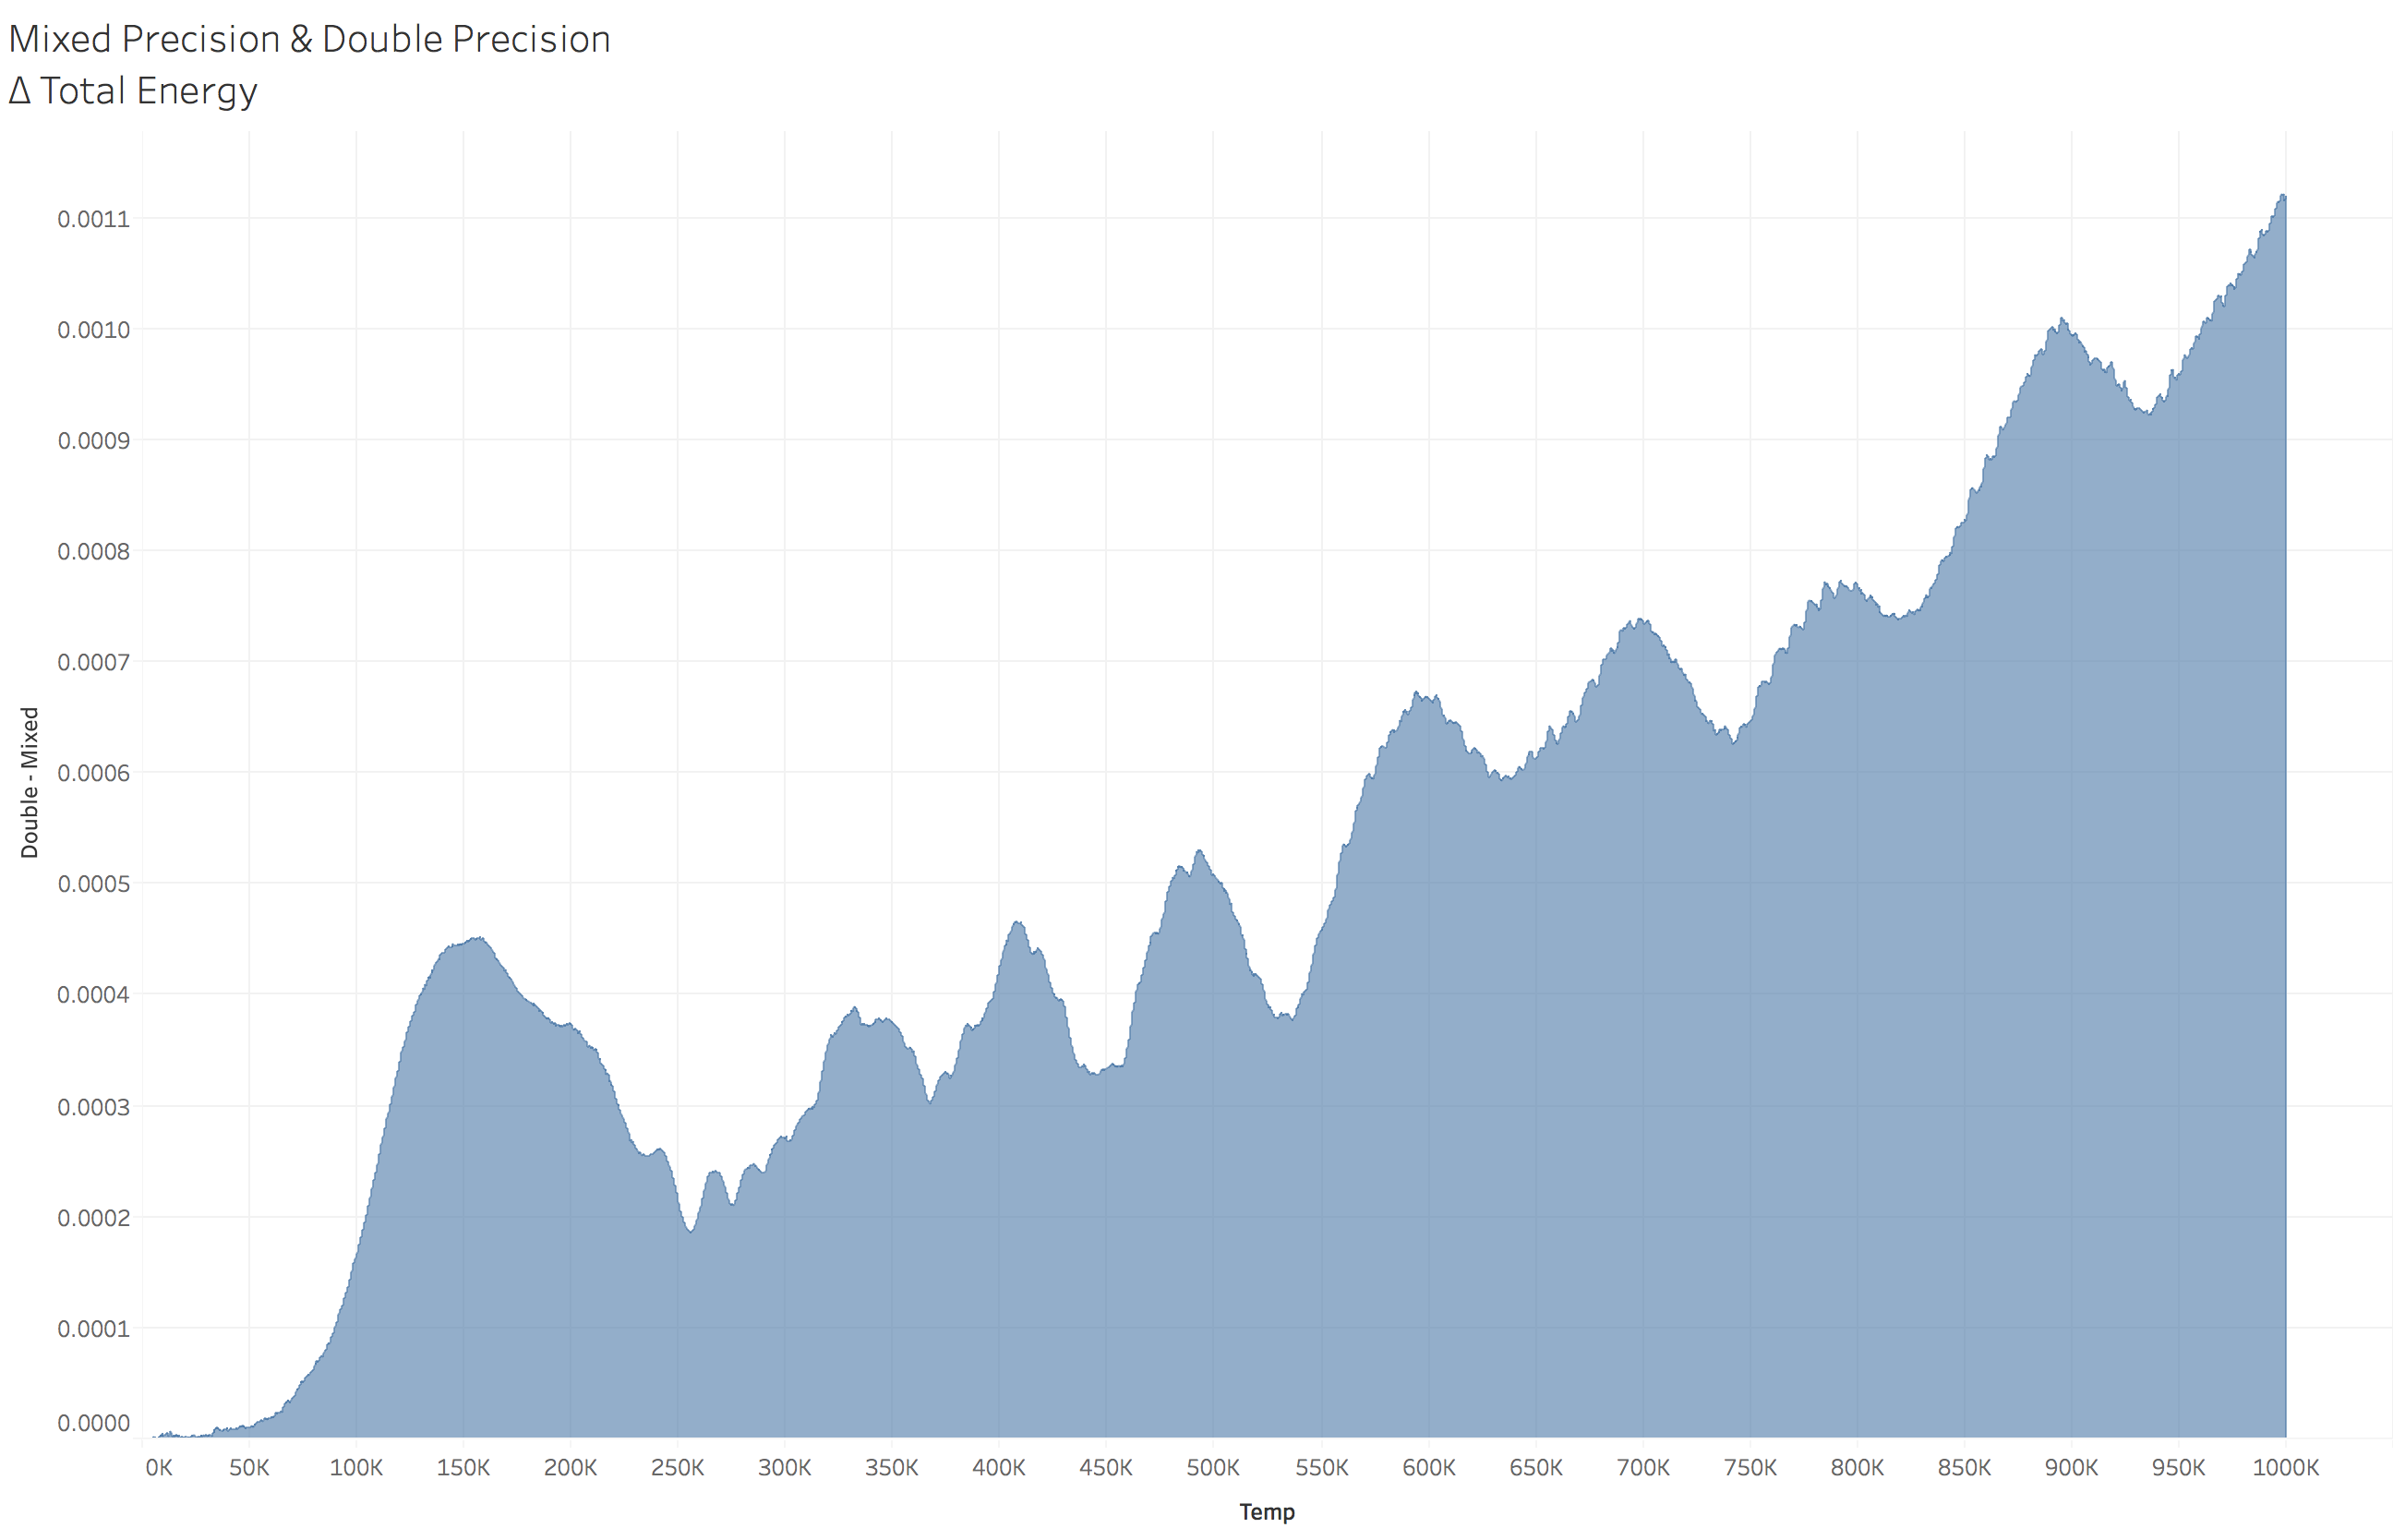
\includegraphics[height=6cm, width=8cm]{Mixed-Double.png}
\caption{Validation of the single precision solver: relative difference between the mixed and double precision solvers for a system of 32,000 atoms for $10^{6}$ timesteps}
\vskip -6pt
\end{figure}


\subsection{Single-Thread Execution}
Using the \texttt{in.tersoff} data set, we ran single-threaded execution tests using four different modes:  Ref, Opt-D, Opt-S, and Opt-M.\\
\textit{Ref:} This is the reference for the tests and the naive LAMMPS distribution, which is performed in double precision.\\
\textit{Opt-D:} This is the most accurate version of the code, performing calculations in double precision.\\
\textit{Opt-S:} This is the least accurate version of the code, performing calculations in single precision but including the scalar optimizations and vectorization.  \\
\textit{Opt-M:} This is a mixed-precision version of the code with the purpose of compromising between speed and accuracy.  It uses single-precision for all calculations except the accumulation operation.\\
We observed speedups of 3.7 between Ref and Opt-D and 4.8 between Ref and Opt-S on the AVX2 instruction set.  On our compute nodes utilizing the AVX512 instruction set, we observed speedups of 3.4 between Ref and Opt-D and 4.3 between Ref and Opt-S. The results of these test runs are shown in Figure 3 and are within the range of speedups shown in the paper for the Haswell architecture, which has similar vector instruction units as our cluster.\\

\begin{figure}
\centering
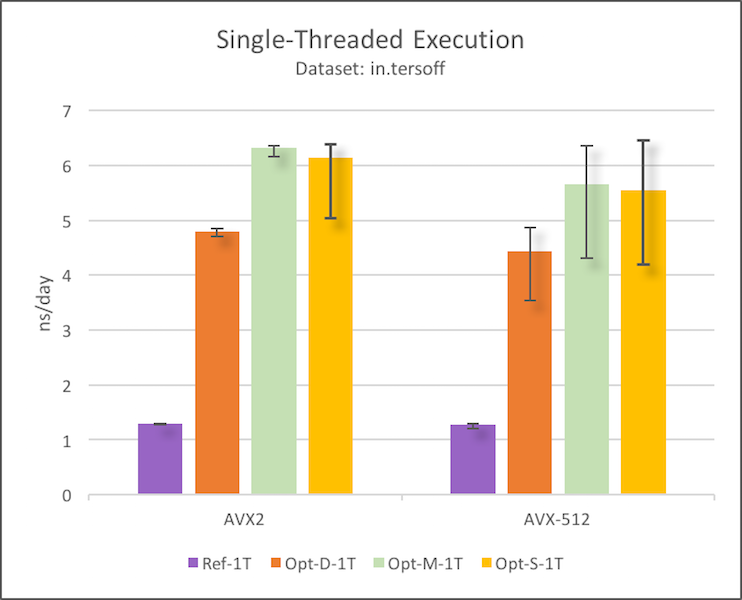
\includegraphics[height=6cm, width=8cm]{SingleThread.png}
\caption{Evaluation of performance portability across CPUs; single-threaded execution for a system of 32,000 atoms.}
\vskip -6pt
\end{figure}

\subsection{Single Node Execution}
We ran two datasets, \texttt{in.tersoff\_bench} and \texttt{in.porter} on the Ref and Opt-M implementation modes.  We ran these tests on a single node with 16 MPI ranks, one rank per node.  Using the \texttt{in.tersoff\_bench} data set we observed speedups of 4.3 on the AVX2 vector set and of 3.76 on the AVX-512 vector set.  These results are shown in Figure 4.  Figure 5 shows observed speedups of 2.01 and 2.28 on the AVX2 and AVX-512 vector sets respectively using the \texttt{in.porter} data set.  The speedups for the \texttt{in.tersoff\_bench} are within the range of speedups for the same tests in the paper.  However, the range of speedups for the \texttt{in.porter} data set are slightly below the range displayed in the paper for similar vector units.

\begin{figure}
\centering
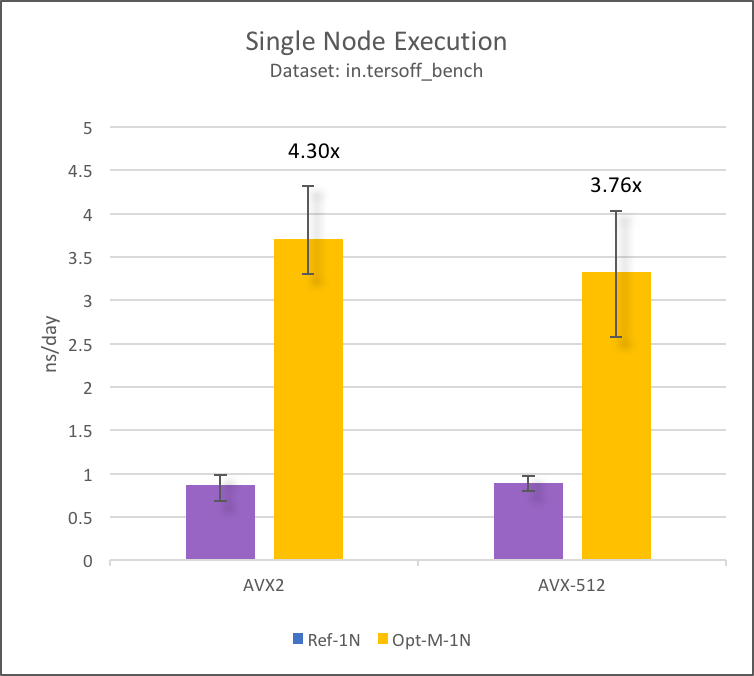
\includegraphics[height=6cm, width=8cm]{SingleNodeBench.png}
\caption{Evaluation of performance portability across CPUs; single-threaded execution for a system of 32,000 atoms.}
\vskip -6pt
\end{figure}

\begin{figure}
\centering
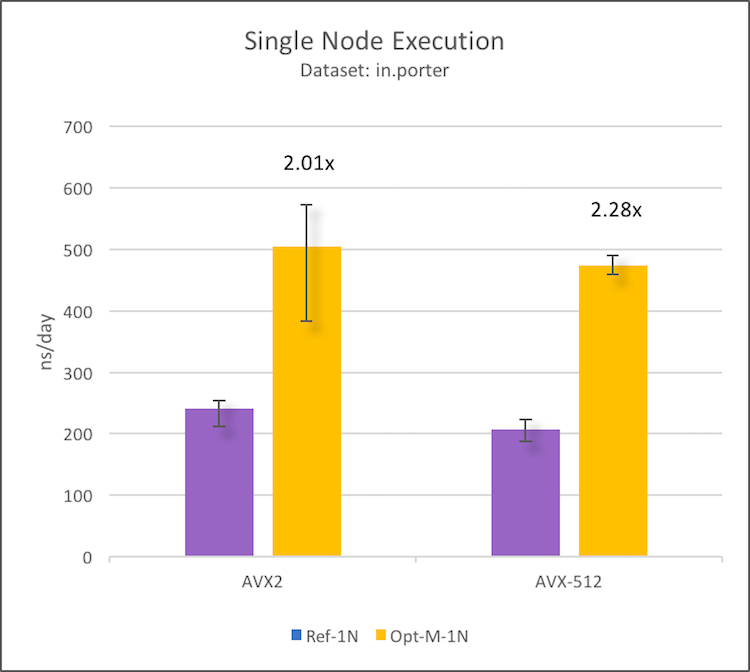
\includegraphics[height=6cm, width=8cm]{SingleNodePorter.png}
\caption{Evaluation of performance portability across CPUs; single-threaded execution.  32,000 atoms.}
\vskip -6pt
\end{figure}


\subsection{Scalability}
The last tests of our reproducibility exercise involved scaling the optimizations on our cluster.  We performed tests using the 
\texttt{in.tersoff\_bench} and \texttt{in.porter} datasets, performing the same tests on one node, two nodes, and four nodes.  On one node we used 16 MPI ranks.  On two nodes we used 32 MPI ranks with 16 ranks per node, and on four nodes we used 64 MPI ranks with 16 ranks per node.  All of these tests were run on our compute nodes, utilizing the AVX512 instruction set.  We ran these tests using the Ref and Opt-M modes.  As shown in Figure 5, the tests on dataset \texttt{in.tersoff\_bench} showed strong scaling across all four nodes.  However, the dataset \texttt{in.porter} did not scale well across the nodes. 


\begin{figure}
\centering
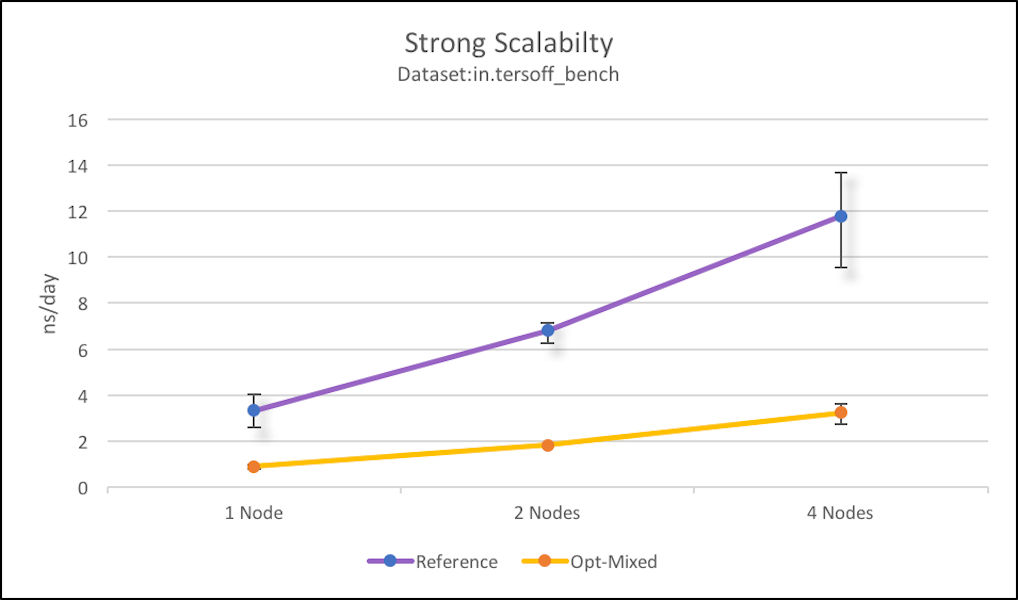
\includegraphics[height=6cm, width=8cm]{ScalingBench.png}
\caption{Optimization results on the SaltFlats cluster using \texttt{in.tersoff\_bench} data set.}
\vskip -6pt
\end{figure}

\begin{figure}
\centering
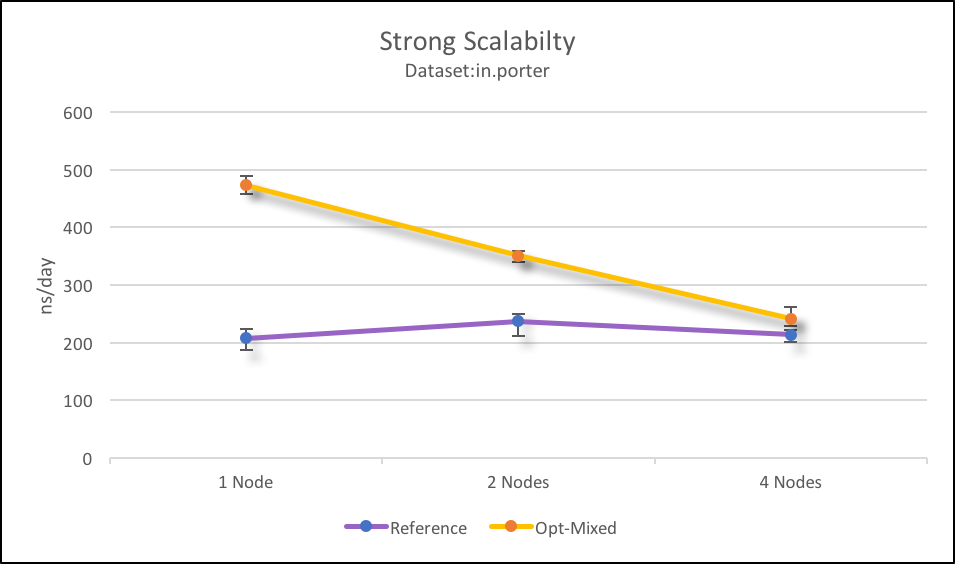
\includegraphics[height=6cm, width=8cm]{ScalingPorter.png}
\caption{Optimization results on the SaltFlats cluster using \texttt{in.porter} data set.}
\vskip -6pt
\end{figure}

\subsection{Conclusion}
We ran numerous tests on four data sets to reproduce the results presented in the paper.  The accuracy test results were not similar to the accuracy test presented by the authors.  The relative difference in our tests were larger by a factor of 50 and increased over the number of timesteps.  The datasets \texttt{in.tersoff} and \texttt{in.tersoff\_bench} displayed speedups similar to the paper and exhibited the portability on our cluster of the optimized LAMMPS code for the Tersoff potential.  The results from the \texttt{in.porter} were not as strong in displaying the portability of the optimized code.  We observed speedups just below the range demonstrated in the paper.  This dataset also did not scale well across our cluster.  Possible reasons include the amount of time spent in communication could overtake the speedups provided by the vectorization and other optimizations, and the size of the neighbor lists could also alter the performance.

We also observed that the speedups did not necessarily improve by using the AVX-512 vector instruction set over using the AVX2 instruction set.  Possible reasons for this include a lower clock speed for the AVX-512 CPUs on our cluster than the AVX2 CPU and other cluster configurations. 

% That's all folks!
\end{document}
